
\section{Introduction}
After going through a bunch of different platforms to work on, we concluded that TensorFlow, using Python, was the most efficient and time-effective way to implement our ideas. This is due to their excellent documentation, numerous examples and a giant welcoming community of enthusiastic developers.


\section{About the Data}
To start off our attempt at implementation, we used a small openly available positive and negative sentiment dataset with 5331 lines of labelled data, for each positive and negative sentiment. We used a basic, Feed-forward Back-propagating Neural Network and focused on it being expandable, flexible and easy to understand and implement. Full Code Link \href{https://github.com/hsaygan/B.Tech-Project}{here.}


\begin{center}
\begin{tabular}{| c |}
\hline
"too much power , not enough puff"\\
"narc is all menace and atmosphere"\\
"an almost unbearably morbid love story"\\
"feels strangely hollow at its emotional core"\\
"enigma is well-made , but it's just too dry and too placid"\\
"it's tough to be startled when you're almost dozing"\\
\hline
\end{tabular}\newline
\caption{Extracts (per line) for Negative Sentiment Dataset}
\end{center}

\begin{center}
\begin{tabular}{| c |}
\hline
"another best of the year selection"\\
"an entertaining , if ultimately minor , thriller"\\
"an almost unbearably morbid love story"\\
"a lovably old-school hollywood confection"\\
"simultaneously heartbreakingly beautiful and exquisitely sad"\\
"a solidly entertaining little film"\\
\hline
\end{tabular}\newline
\caption{Extracts (per line) for Positive Sentiment Dataset}
\end{center}


The entire data consists of 2 files, namely Positive.txt and Negative.txt, both of which can be extracted from \href{https://pythonprogramming.net/static/downloads/machine-learning-data/pos.txt}{Positive.txt} and \href{https://pythonprogramming.net/static/downloads/machine-learning-data/neg.txt}{Negative.txt} links.

\section{Data Preprocessing}
The data, as one can see, is in natural language and is completely unstructured. Therefore, to apply any implementation, first we need to process it in an organized format to make it structured.
To restructure this data, we used various Library like NLTK, NumPy, Pandas, Pickle etc. The preprocessing follows the given structure
\begin{itemize}
  \item Creating Lexicon
  \item Creating Vectors
  \item Adding Labels
  \item Creating Featuresets
  \item Exporting Final Data
\end{itemize}

\subsection{Creating Lexicon}
First we created Lexicon, which is basically a dictionary for all the words that appear in all the lines in a file. Tokenizer extracts words from each line of the file, removing unnecessary words like "the", "and" etc. which do not contribute to sentiments or quality of the line. We also used Lemmatizer to eliminate words which infer the same (ex. "cat" and "cats" can be treated as one). Creating Lexicon gives us the full discovery of all the words occurring in both the files

\subsection{Creating Vectors}
After creating the Lexicon, we form a NumPy array (of Zeros initially) for each and every line of both the files. This array represents the words that are present in that particular line with respect to the lexicon. This means, that the array is a vector, which has 1 (or $>$ 1) values due to words occurring in that line, at the same index as of the lexicon's.

\begin{verbatim}
Let the Lexicon be:
    lex = {"Cat", "Ball", "Mouse", "Pizza"}
Also, let a line be:
    line = "Cat ate the mouse"
Therefore, it's vector will be:
    vec = [1, 0, 1, 0]

Note: Actual Size of Lexicon = 423
\end{verbatim}

\subsection{Adding Labels}
Vectors, after being created for each line for both the files, are then combined with their labelled sentiment. ie. "[1,0]" for Positive Sentiment, and "[0,1]" for Negative Sentiment.
Therefore, the vector now transforms into a 2 dimentional aspect, one containing the vector of words in the line, and the other containing the label it carries.

\begin{verbatim}
Let a vector be:
    vec = [1, 0, 1, 0]
Now let's say that it was in the positive.txt file, therefore it will be labbeled as [1,0]
    final_vec = [[1,0,1,0], [1,0]]
\end{verbatim}

\subsection{Creating Featuresets}
All the final vectors formed are combined in one giant object, named 'featureset'. Note that this object contains all the lines in both the files in vector forms along with their labels.
After creating this object, we randomize entry. This is to ensure in the future that when the Neural Network will be training on this data, It won't be trained to the extreme for one sentiment (More on this in later sections).
After Randomizing, we split the object in 4 Objects, diving them to form training and testing data. The code is self explanatory.

\begin{verbatim}
    train_x = list(features[:,0][:-testing_size])
    train_y = list(features[:,1][:-testing_size])
    test_x = list(features[:,0][-testing_size:])
    test_y = list(features[:,1][-testing_size:])
\end{verbatim}

\subsection{Exporting Final Data}
After the division of the featureset into the 4 aforementioned objects, the objects are are encapsulated using the 'Pickle' Library, and are exported. Pickle data are converted from python objects to byte stream. It helps serialize all the data, and makes storage and access of python objects easier.

\section{Building The Neural Network}
We used Neural Networks due to it's expandability and flexibility regarding fitting data points and it's accuracy over larger datasets. The standard Neural Network Model we build consisted of 1 Input, 2 Hidden, 1 output layer. Number of nodes in Input layer is decided by the length of 'train-x' features from the pickle. Output Layer consists of a single node. Since it's a classification problem (whether a line exhibits positive or negative sentiment) the output node has 2 classes, one for each sentiment.

\subsection{Neural Network Model}
In this fully connected Neural Network, each node is connected to all the nodes in the layer before and after it's own layer. The diagram makes it easier to visualize. Each connection between 2 nodes has a weight and a bias value associated with it, which is initialized to random numbers. We also used Rectified Linear (or ReLu) as an activation function for each connection. 

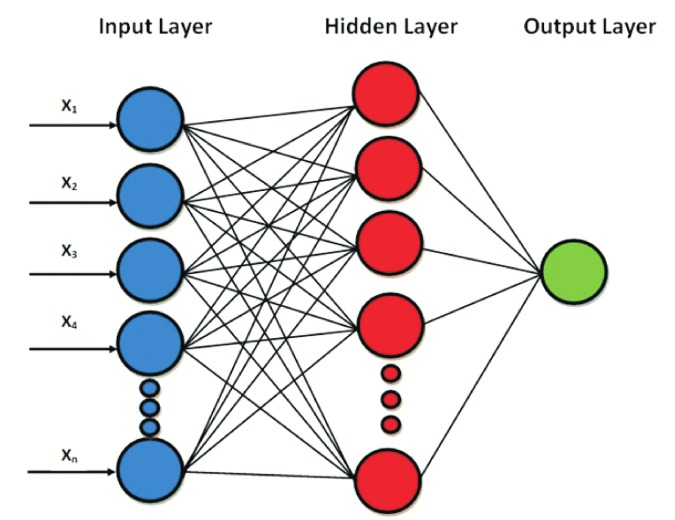
\includegraphics[scale=0.4]{Figures/nn_model.jpg}

\subsection{Feed-forward and Back-propagation}
After the Neural Network Model is built, we set it up to train it with our data. We used Softmax Cross Entropy with Logits, to reduce cost and AdamOptimizer instead of classical stochastic gradient which is a combination of Adaptive Gradient Algorithm(AdaGrad) and Root Mean Square Propagation (RMSProp), and a standard in TensorFlow. We Then trained the Model in Batches of 100 lines per batch. Do Note that TensorFlow is a library which handles back propogation all by itself with the provided model in a given session. Thus, the labour intensive part was handled by the library itself.

\begin{verbatim}
#This is the session's code where Neural Network is Trained
with tf.Session() as sess:
        sess.run(tf.global_variables_initializer())
        for epoch in range(hm_epochs):
            epoch_loss = 0
            i=0
            while i < len(train_x):
                start = i
                end = i + batch_size
                batch_x = np.array(train_x[start:end])
                batch_y = np.array(train_y[start:end])
                
                #Sess.run handles backpropagation and reduces the cost of the Model
                _, c = sess.run([optimizer, cost], feed_dict={x: batch_x, y: batch_y})
                epoch_loss += c
                i += batch_size
            print('Epoch', epoch+1, 'completed out of',hm_epochs,'loss:',epoch_loss)
        correct = tf.equal(tf.argmax(prediction, 1), tf.argmax(y, 1))
        accuracy = tf.reduce_mean(tf.cast(correct, 'float'))

#Epoch is the number of times the Model is being trained by the same data
\end{verbatim}

\section{Testing and Results}
Training and Testing gave us alot of insights other than accuracy. Following subsections shows extracted and plotted data of cost and also shows the result of our experimentation on the Neural Network Model by modifying multiple parameters like the Number of Epochs, Number of Hidden Layers, Nodes in the Hidden Layers etc. All of the results can easily be visualized with the Graphs below.

\subsection{Lexicon Dictionary and Input}
After the preprocessing of the data, we get the final lexicon as well as featuresets and labels for both, testing and training data.

\begin{verbatim}
Length of Lexicon:  423
Lexicon: 
 ['american', 'since', 'been', 'when', 'screen', 'both', 'just',
 'character', 'part', 'charm', 'obvious', 'too', 'sense' ...
 'boring', 'dull']
 
#Below are examples of one of each, of the following-
train_x (Training Data): 
[1, 1, 2, 1, 1 ...  0, 0]

train_y (Training Label):
[1, 0]

test_x (Testing Data): 
[0, 0, 0, 2, 0, 0 ... 1, 0]

test_y (Testing Label):
[0,1]
\end{verbatim}


\subsection{Cost Reduction}
The whole point of Neural Network (or Gradient Descent) is to minimize the Cost function efficiently. Here we see the Neural Network Model's improved cost after each individual epoch. The figure resembling a hyperbola suggests a good backpropagation and reasonably efficient Neural Network Model.

\begin{tikzpicture}
\begin{axis}[
    title={Cost per Epoch},
    xlabel={Epoch},
    ylabel={Cost},w
    xmin=0, xmax=25,
    ymin=0, ymax=8000,
    xtick={1,2,3,4,5,6,7,8,9,10,11,12,13,14,15,16,17,18,19,20,21,22,23,24,25},
    ytick={8000, 5000, 2000, 1000, 100, 50},
    legend pos=north west,
    ymajorgrids=true,
    grid style=dashed,
]

\addplot[
    color=blue,
    mark=square,
    width=\textwidth
    scale=1.
    ]
    coordinates {
    (1,7640.895782470703)(2,4403.4900550842285)(3,3175.1762590408325)(4,2472.2888412475586)(5,1984.7782068252563)(6,1614.7941551208496)(7,1317.6516003608704)(8,1086.8701810836792)(9,914.826991558075)(10,804.6651692390442)(11,704.8594558238983)(12,577.8208487033844)(13,449.56429040431976)(14,379.81100302934647)(15,334.5576722025871)(16,297.5162614732981)(17,280.0793870985508)(18,245.94800680875778)(19,204.7364508509636)(20,130.01248725503683)(21,89.33359460160136)(22,69.76632069051266)(23,56.63669146038592)(24,46.57956535532139)(25,37.51003663055599)
    };
    \legend{Cost}
\end{axis}
\end{tikzpicture}


\subsection{Varying Epochs}
Epochs are the number of loops the training data is feeded into the Neural Network Model. Epoch iterations are a key element to get a Neural Network more precise output, with reference to the training data. Here, we vary epoch from 10 to 50, keeping everything else constant, to get an overview of the varied accuracy with respect to number of Epochs.

\begin{center}
\begin{tabular}{| c | c |}
\hline
Number of Epochs & Variable\\
Number of Hidden Layers & 2\\
Number of Hidden Nodes & 400, 200\\
\hline
\end{tabular}
\end{center}

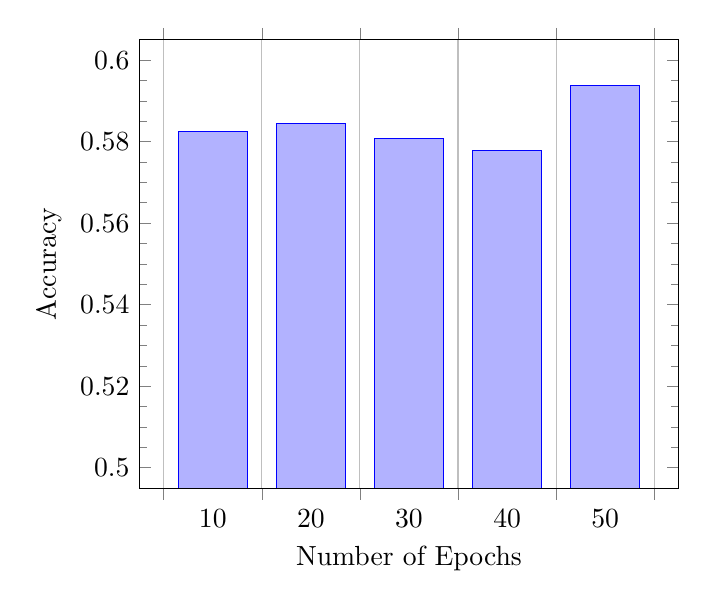
\begin{tikzpicture}
\begin{axis}[
    ymin=0.5, ymax=0.6, ylabel=Accuracy, xlabel=Number of Epochs, minor y tick num = 3, area style, xmin=10, xmax=60,
    x tick label style={/pgf/number format/1000 sep=},
	enlargelimits=0.05,	ybar interval=0.7,
    ]
\addplot+[ybar interval,mark=no] plot coordinates { (10, 0.5825516) (20, 0.5844278) (30, 0.5806754) (40, 0.5778612) (50, 0.5938086) (60,0)};
\end{axis}
\end{tikzpicture}

%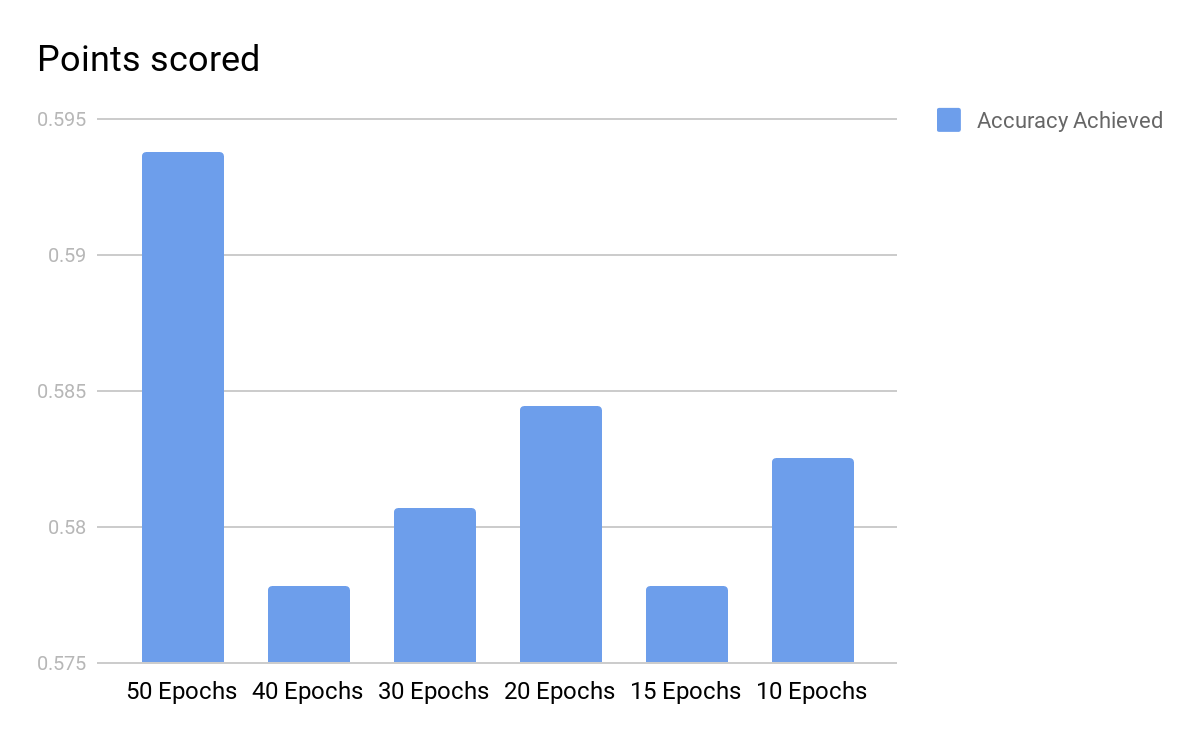
\includegraphics[scale=0.3]{epoch.png}

\subsection{Varying Hidden Layer Nodes}
Number of hidden layer builds up complexity of the Neural Network Model. More the number of hidden layer's nodes, the more inter-node connections are required, ie. more Weights and Biases. This elevation in complexity shall help in complex sentence's determination of sentiments, but requires more computation in creating the model.

\begin{center}
\begin{tabular}{| c | c |}
\hline
Number of Epochs & 25\\
Number of Hidden Layers & 3\\
Number of Hidden Nodes & Variable\\
\hline
\end{tabular}
\end{center}

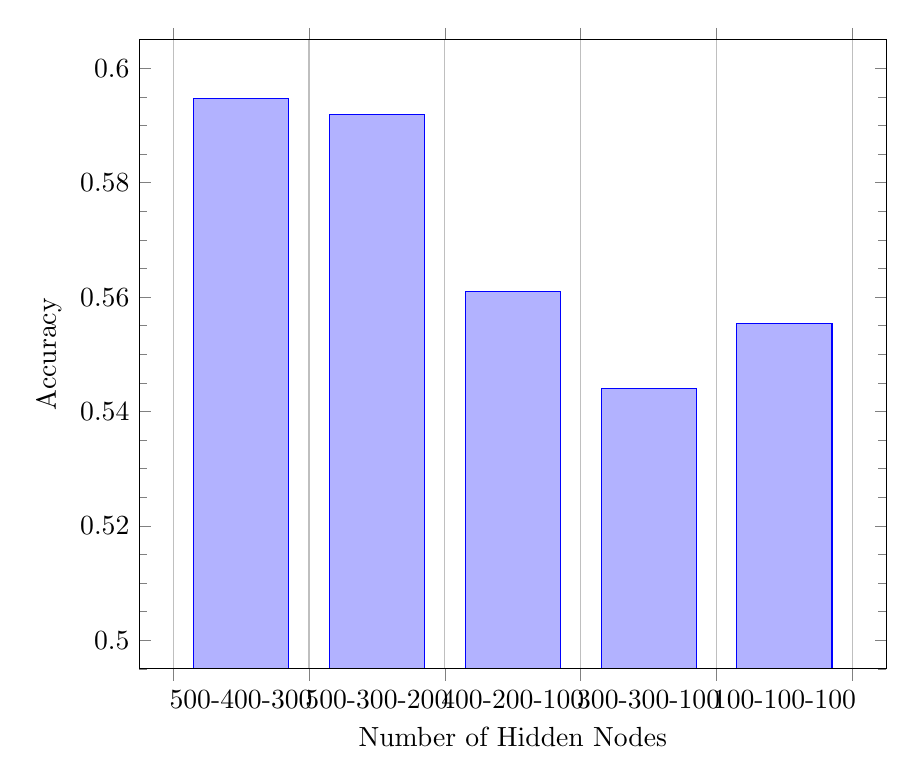
\begin{tikzpicture}
\begin{axis}[
    scale=0.9, ymin=0.5, ymax=0.6, ylabel=Accuracy, xlabel=Number of Hidden Nodes, minor y tick num = 3, area style, width=\textwidth,
	enlargelimits=0.05,	ybar interval=0.7,
	xticklabel style={text height=1.5ex},
	symbolic x coords={500-400-300,500-300-200,400-200-100,300-300-100, 100-100-100, 50-40-20}
    ]
\addplot+[ybar interval,mark=no] plot coordinates { (500-400-300, 0.5947467) (500-300-200, 0.5919325) (400-200-100, 0.5609756) (300-300-100, 0.54409003) (100-100-100, 0.5553471) (50-40-20, 0.54971856)};
\end{axis}
\end{tikzpicture}

%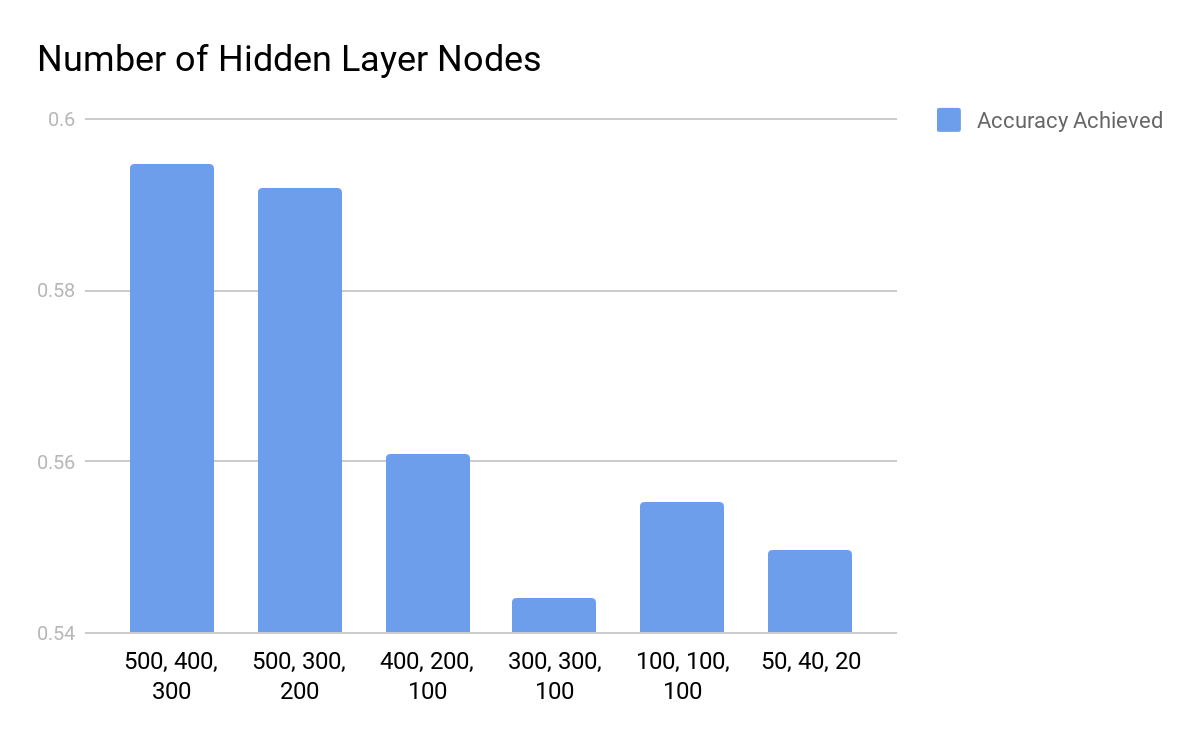
\includegraphics[scale=0.3]{hlnodes.png}

\subsection{Varying Number of Hidden Layers}
Similar to varying the number of hidden nodes, adding more hidden layers contribute significantly in making the model more complex. However it is evident from the resulting graph that more layers results in less accuracy, since more time will be needed to train the extra variables induced due to variable hidden layers.

\begin{center}
\begin{tabular}{| c | c |}
\hline
Number of Epochs & 25\\
Number of Hidden Layers & Variable\\
Number of Hidden Nodes & 500, 300, 200\\
\hline
\end{tabular}
\end{center}

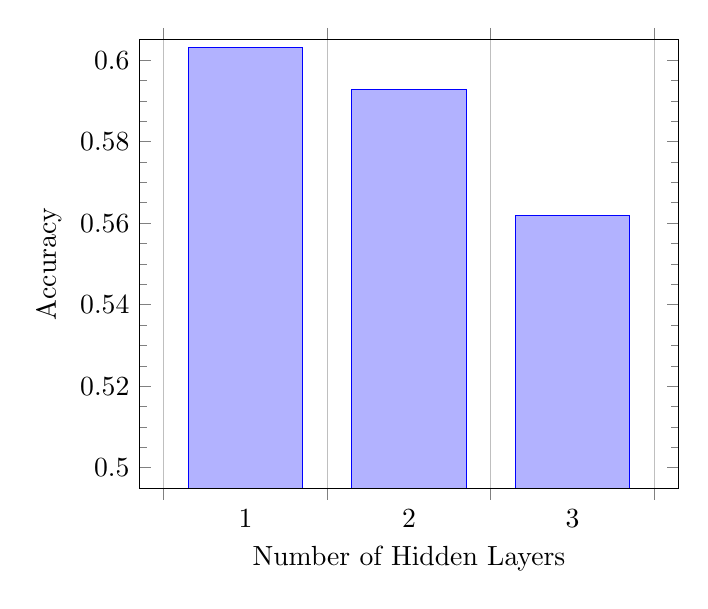
\begin{tikzpicture}
\begin{axis}[
    ymin=0.5, ymax=0.6, ylabel=Accuracy, xlabel=Number of Hidden Layers, minor y tick num = 3, area style,
    x tick label style={/pgf/number format/1000 sep=},
	enlargelimits=0.05,	ybar interval=0.7, xmin=1, xmax=4,
    ]
\addplot+[ybar interval,mark=no] plot coordinates { (1, 0.60318947) (2, 0.5928518) (3, 0.5619325) (4,0)};
\end{axis}
\end{tikzpicture}


%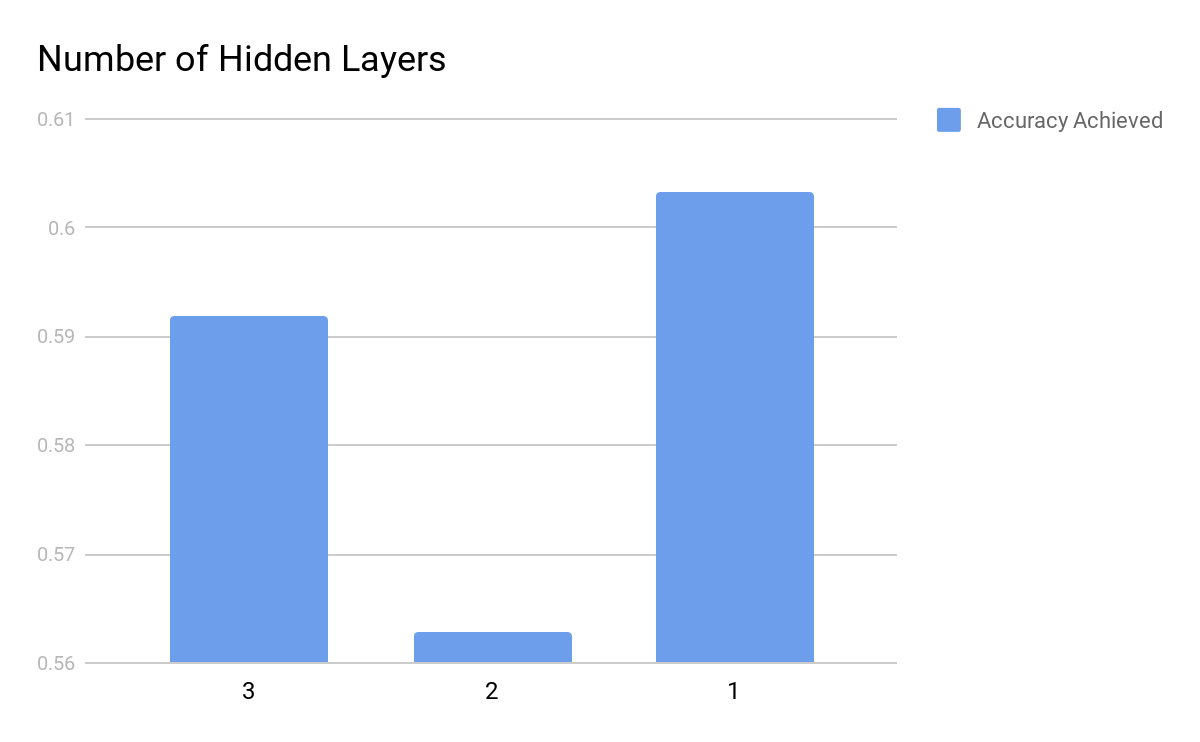
\includegraphics[scale=0.3]{nhiddenlayers.png}

\section{Conclusion}
From the above results we can conclude that the effect of either of the parameters is not that significant, as it's in the margin of error of the random value of the weights and biases in the initialization process since the Standard Deviation of the random tensor is 1.0. 

\begin{verbatim}
tf.random_normal
(
    shape,
    mean=0.0,
    stddev=1.0,
    dtype=tf.float32,
    seed=None,
    name=None
)
\end{verbatim}

Along with this, we can conclude that most of the deviations of accuracy, which was withing +-5, is not note-worthy.\newline
Since Neural Network's heart lies in it's data, we strive to get more data to train our Neural Network. In the next chapter, we move from data  of just 5331 lines of unstructured Natural Language, to 1.6 Million lines of unstructured labelled Data from Tweets.